\documentclass{article}
\usepackage[top=2cm,bottom=2cm,left=2cm,right=3.5cm]{geometry}

\usepackage[utf8]{inputenc}
\usepackage{amssymb}
\usepackage{hyperref}
\usepackage{multirow}
\usepackage[most]{tcolorbox}
\tcbuselibrary{skins,breakable}

\newtcolorbox{callout}[2][]{breakable,sharp corners, skin=enhancedmiddle jigsaw,parbox=false,
boxrule=0mm,leftrule=2mm,boxsep=0mm,arc=0mm,outer arc=0mm,attach title to upper,
after title={.\ }, coltitle=purple,colback=purple!10,colframe=purple, title={#2},
fonttitle=\bfseries,#1}

\newtcolorbox{warning}[2][]{breakable,sharp corners, skin=enhancedmiddle jigsaw,parbox=false,
boxrule=0mm,leftrule=2mm,boxsep=0mm,arc=0mm,outer arc=0mm,attach title to upper,
after title={!\ }, coltitle=red,colback=red!10,colframe=red, title={#2},
fonttitle=\bfseries,#1}

\newtcolorbox{esempio}[2][]{breakable,sharp corners, skin=enhancedmiddle jigsaw,parbox=false,
boxrule=0mm,leftrule=2mm,boxsep=0mm,arc=0mm,outer arc=0mm,attach title to upper,
after title={:\ }, coltitle=blue,colback=blue!10,colframe=blue, title={#2},
fonttitle=\bfseries,#1}

\newcommand{\na}[0]{\ensuremath {\overset{N}{\rightarrow}}}
\newcommand{\rl}[3]{\inference{#1}{#2}\text{ #3}}
\newcommand{\bop}[0]{\ensuremath\oplus}
\newcommand{\appl}[2]{\ensuremath(#1)\ #2}
\newcommand{\st}[3][]{\ensuremath{\displaystyle\frac{#3\hfill}{#2\hfill} \text{#1}}}
\newcommand{\N}{\ensuremath \mathbb N}
\newcommand{\I}{\ensuremath \mathbb I}
\newcommand{\lam}[2]{\ensuremath{\lambda#1.#2}}
\newcommand{\inl}[0]{\ensuremath{\ inl\ }}
\newcommand{\inr}[0]{\ensuremath{\ inr\ }}
\newcommand{\case}[3]{\ensuremath{\text{case}#1\ \text{of}\ \left|\begin{aligned}& #2\\ & #3\end{aligned}\right.}}
\newcommand{\Da}[0]{\ensuremath{\Downarrow}}
\newcommand{\while}[2]{\ensuremath{\text{while }#1\text{ do }#2\text{ end}}}
\newcommand{\for}[3]{\ensuremath{\text{for }i=#1\text{ to }#2\text{ do }#3\text{ end}}}
\newcommand{\mE}[0]{\ensuremath{\mathbb{E}}}
\newcommand{\pair}[1]{\ensuremath{\langle#1\rangle}}
\newcommand{\V}{\ensuremath{\mathcal{V}}}
\newcommand{\cE}{\ensuremath{\mathcal{E}}}
\newcommand{\cD}{\ensuremath{\mathcal{D}}}
\newcommand{\cF}{\ensuremath{\mathcal{F}}}
\newcommand{\IF}[0]{\ensuremath {\text{ if }}}
\newcommand{\THEN}[0]{\ensuremath {\text{ then }}}
\newcommand{\ELSE}[0]{\ensuremath {\text{ else }}}
\newcommand{\AND}[0]{\ensuremath {\text{ and }}}
\newcommand{\OR}[0]{\ensuremath {\text{ or }}}
\newcommand{\unpack}[3]{\ensuremath{\text{unpack } #1 \text{ as }\langle #2 \rangle\text{ in }#3}}
\newcommand{\pack}[2]{\ensuremath{\text{pack } \pair{#1} \text{ as } #2 }}
\newcommand{\te}[1]{\text{#1}}
\newcommand{\ls}[0]{\ensuremath{\leadsto^{*}}}
\newcommand{\LET}[0]{\ensuremath{\text{ let }}}
\newcommand{\TIN}[0]{\ensuremath{\text{ in }}}
\newcommand{\NEW}[0]{\ensuremath{\text{ new }}}

\usepackage[parfill]{parskip}
\usepackage{marginnote}
\usepackage{ulem}

\usepackage{graphicx}
\usepackage{algorithm2e}

\title{Automated Reasoning and Formal Verification}
\author{Diego Oniarti}
\date{Anno 2024-2025}

\begin{document}

\maketitle
\tableofcontents

\section{25-02-2025}
\subsection*{intro}
Slides will be on his \href{https://disi.unitn.it/rseba/DIDATTICA/arfv2025/}{webpage} along with the recordings.

The exam will consist of a script and an oral exam on the topics of the whole course.

\subsection*{boolean/propositional logic}
A propositional \textbf{formula} can be:
\begin{itemize}
    \item $\top$, $\bot$
    \item Propositional \textbf{atoms} $A_1, A_2, \dots, A_n$
    \item A combination of other formulas. If $\varphi_1$ and $\phi_2$ are formulas, so are:
        \begin{itemize}
            \item $\neg \varphi_1$
            \item $\varphi_1\wedge\phi_2$
            \item $\varphi_1\vee\phi_2$
            \item $\varphi_1\to\phi_2$
            \item $\varphi_1\leftarrow\phi_2$
            \item $\varphi_1\leftrightarrow\phi_2$
            \item $\varphi_1\oplus\phi_2$
        \end{itemize}
\end{itemize}

We define a function $Atoms(\varphi)$ representing the set $\{A_1,\dots,A_n\}$ of atoms in $\phi$

A \textbf{clause} is a disjunction of literals $\bigvee_j l_j$ or $(A_1\vee \neg A_2 \vee ...)$

A \textbf{cube} is a conjunction of literals $\bigwedge_j l_j$ or $(A_1\wedge \neg A_2 \wedge ...)$

\subsection*{trees and DAGS}
A tree is a natural representation of an expression, but in the worst cases it can grow exponentially. The same information about the formula can be conveyed by a \textit{Directed Acyclic Graph}, which can grow linearly in size.

\subsection*{Total Truth Assignment}
They can also be abbreviated as \textit{Total Assignment}.\\
A total truth assignment $\mu: Atoms(\varphi)\mapsto\{\top,\bot\}$ represents \textit{one} possible state of the formula.

\subsection*{Partial Truth Assignment}
A partial truth assignment $\mu: \mathcal A \mapsto\{\top,\bot\}, \mathcal A\subset Atoms(\varphi)$ represents $2^k$ total assignments, where $k$ is the number of unassigned literals.

$\mu$ defined for total and partial truth assignments a can be seen as a set of literals (positive and negative ones) or a formula.

\subsection*{Set of models}
$M(\varphi) \triangleq \{\mu | \mu\models\phi\}$ is the set of all models of $\phi$.

\subsection*{Properties}
\begin{itemize}
    \item $\varphi$ is \textit{valid} if every $\mu$ models $\phi$
    \item $\varphi\ \te{valid} \iff \neg\phi\te{ unsatisfiable}$
    \item $\alpha\models\beta \iff \alpha\to\beta\te{ valid}$\marginnote{Deduction theorem}
    \item $\alpha\models\beta \iff \alpha\wedge\neg\beta\ \te{not satisfiable}$\reversemarginpar\marginnote{corollary}
\end{itemize}

\subsection*{Equivalence and Equi-satisfiability}
$\alpha$ and $\beta$ are \textit{equivalent} if $\forall \mu.\mu\models\alpha\iff\mu\models\beta$.\\
In other terms, $M(\alpha)=M(\beta)$.

\textbf{Equi-satisfiability} $M(\alpha)\neq\emptyset \iff M(\beta)\neq\emptyset$. This property is mostly used when applying transformations to formulas $\beta\triangleq T(\alpha)$.

Transformations can be \textit{validity preserving} if they preserve the validity of the formula they're being applied to, or \textit{satisfiability preserving} if they preserve its satisfiability.

\subsection*{Shannon's expansion}
$$\exists v.\varphi := \phi|v=\bot \vee \phi|v=\top$$ The existential is a disjunction between two possible formulas. One where $v$ is set to true, and one where it is set to false.
$$\forall v.\varphi := \phi|v=\bot \wedge \phi|v=\top$$ The universal one is similar, with a conjunction between the two.

\subsection*{Polarity of subformulas}
Polarity is a metric defined for each subformula of a formula $\varphi$ that tells us under how many nested negations it occurs. It can either be positive, negative, or both in some cases.\\
The recursive rules to determine the polarity are shown in the image below
\begin{center}
    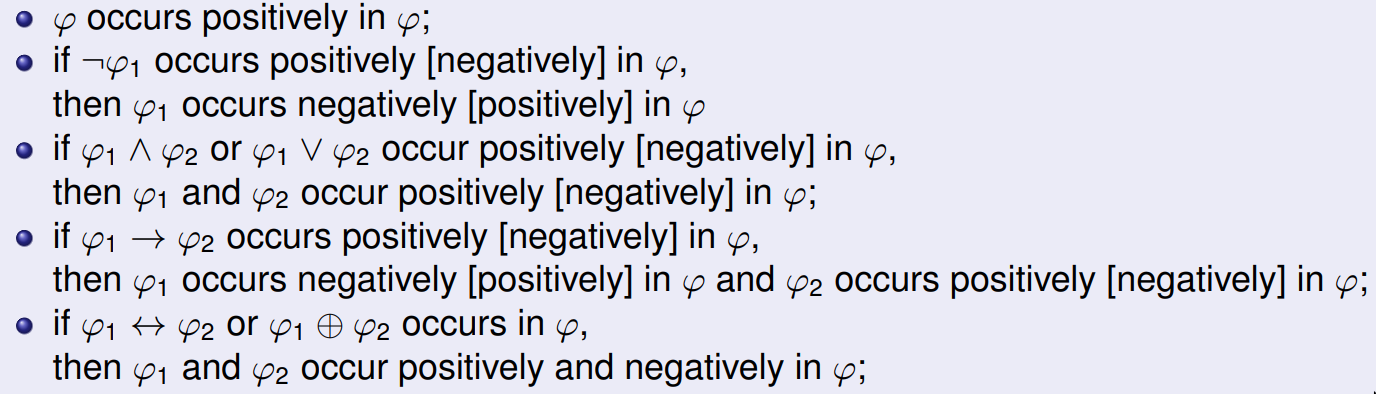
\includegraphics[width=0.8\linewidth]{images/polarity.png}
\end{center}

If we assume $\top=1,\bot=0$ we can also see the polarity of a subformula as "how much it contributes to the overall value of the formula".

\section{Normal forms}
\subsection{Negative Normal Form - NNF}
A negative normal form is a formula in which each negations has been pushed down to the atoms. This implies that every subformula in $NNF(\varphi)$ has positive polarity.

\paragraph{Properties}
\begin{itemize}
    \item Every formula can be made into negative normal form
    \item NNF transformation preserves equivalence
\end{itemize}

\subsection{Conjunctive Normal Form - CNF}
\begin{gather*}
\bigvee_{i=1}^L \bigwedge_{j=1}^{K_i} l_{ij} \\
(l_{11} \wedge l_{12})\vee(l_{21} \wedge l_{22} \wedge l_{23})\vee(...)\vee...
\end{gather*}

Every formula can be converted in \textit{Conjunctive Normal Form}, but there are different ways to do so.

\subsubsection{Naive CNF conversion}
The more intuitive and straightforward method consist of:
\begin{enumerate}
    \item Expanding implications and equivalences
    \item Pushing down negations like in NNF
    \item Recursively applying DeMorgan's rule to get the CNF shape
\end{enumerate}

This method produces a CNF that is \underline{equivalent} to the original formula and \underline{has the same atoms}. It is however rarely used in practical applications because it can be up to \uwave{exponentially} larger than the original formula.

\subsubsection{Labeling CNF conversion}
This is a more efficient \textit{bottom-up} approach, which can be executed while parsing the expression.\\
The main idea is that of introducing new variables that serve as "\textit{labels}" for each subformula. The smaller formulas can be converted to CNF with the naive approach, and then assembled through the labels.

This method introduces new atoms, but $\exists(B_1,\dots,B_k).CNF_l(\varphi)\ \te{equiv}\ \phi$ where $B_1,\dots,B_k$ are the newly introduced variables. This means that $\phi$ and $CNF_l(\phi)$ are equisatisfiable.

The representation obtained from the $CNF_l$ can be reduced  further in size by using polarization to change some implications around.

\section{Basic SAT-solving techniques}
\begin{esempio}{Example}
    A classic problem is that of checking a query under a (usually much larger) knowledge base. This problem can be reduced to SAT. $KB\models\alpha$ or $M(KB)\subseteq M(\alpha)$
    \begin{align*}
        KB\models \alpha \iff SAT(KB \vee \neg \alpha) = false
    \end{align*}
\end{esempio}

\subsection{Intro - Unit propagation}
\paragraph{Resolution rule} Deduction of a new clause from a pair of clauses with exactly one incompatible variable (which is called the "\textit{resolvent}").
\begin{align*}
    (a\vee b\vee c) \wedge (d\vee e\vee \neg c) = (a\vee b\vee d\vee e)
\end{align*}

\paragraph{Removal of valid clauses}
If a clause is valid (always true) it can be removed from the formula.

\paragraph{Clause subsumption}
If a clause appears on its own and inside another clause, we can remove the second, bigger, clause.

\paragraph{Unit resolution}
Having a clause composed of a single literal forces said literal to be true. This means we can remove all instances of the negated literal.

\paragraph{Unit subsumption}
Like clause subsumption but with a literal instead of a clause

These unit propagation rules can happen in a chain. After modifying the formula once we can create new unary clauses for example.

\subsection{Resolution algorithm}
\RestyleAlgo{ruled}
\begin{algorithm}
    \caption{Resolution algorithm}
    Assume input is in CNF\;
    $\varphi$ is a set of clauses\;
    \CommentSty{//Search for a \textit{refutation} of $\varphi$}\;
    \Repeat{
        a false clause is generated $\vee$ the rule is not applicable
    }{
        apply resolution rule to pairs of clauses\;
    }
\end{algorithm}
This algorithm is correct and complete, but operates in exponential memory and is time inefficient.

\subsection{Tableaux}
Search assignments satisfying $\varphi$ by applying \textit{elimination rules} on its connectors.\\
Try to be clever and put put smaller clauses first in the branching order.

\section{LAB 1}
\subsection{DIMACS}
Dimacs is the standard format for representing SAT problems.
\paragraph{File structure}
\begin{itemize}
    \item Comments start with 'c'
    \item header of the form 'p cnf 7 8'
        \begin{itemize}
            \item 7: number of variables
            \item 8: number of clauses
        \end{itemize}
    \item 1 clause for line of form "1 -2 0"
        \begin{itemize}
            \item trailing 0 is a constant
            \item 1 first variable
            \item -2 second variable, negated
        \end{itemize}
\end{itemize}

\paragraph{command}
\texttt{mathsat -input=dimacs -model file.cnf}\\
\texttt{-model} tells it to provide a model, otherwise it gives a yes/no answer

\end{document}
